\documentclass[fontsize=11pt]{article}
\usepackage{amsmath}
\usepackage[utf8]{inputenc}
\usepackage[margin=0.75in]{geometry}
\usepackage[round]{natbib}
\usepackage{url}
\usepackage{graphicx}
\usepackage{svg}
\usepackage{subcaption}
\usepackage{booktabs}
\usepackage{multirow}
\usepackage{tabularx}
\graphicspath{ {./images/} }
\bibliographystyle{unsrtnat}

\title{CSC111 Final Project\\ A Graph is worth $2^{|V|}$ Words: GraphBRAIN}
\author{Pranjal Agrawal, Rishit Dagli, Shivesh Prakash, Tanmay Shinde}
\date{Friday, March 26, 2023}

\begin{document}
\maketitle

\section*{Problem Description and Research Question}

The blood$-$brain barrier is a protective layer that separates the brain from the rest of the body’s circulatory system. This barrier is highly selective and prevents solutes in the circulating blood from non-selectively crossing into the extracellular fluid of the central nervous system where neurons reside \citep{daneman2015blood}.

To be effective as therapeutic agents, centrally-acting drugs (central to the brain) must cross the blood-brain barrier. Conversely, to be devoid of unwanted central nervous system effects, peripherally acting drugs (peripherally to the brain) must show limited ability to cross the blood-brain barrier. In both cases, the blood-brain barrier permeability of drug candidates must be known. However, the experimental determination of brain-blood partitioning is difficult, time-consuming, and expensive and not suitable to screen large collections of chemicals \citep{thai2020fast}. A broadly applicable method for predicting the blood$-$brain barrier permeation of candidates at an early stage of discovery would have a great impact on drug research and development. 

The heavily restricting barrier capacity allows BBB ECs to tightly regulate CNS homeostasis, which is critical to allow for proper neuronal function, as well as protect the CNS from toxins, pathogens, inflammation, injury, and disease. The restrictive nature of the BBB provides an obstacle for drug delivery to the CNS, and, thus, major efforts have been made to generate methods to modulate or bypass the BBB for delivery of therapeutics \citep{daneman2015blood}.

Entry into the brain is a complex phenomenon that depends on multiple factors. It is known that relatively lipophilic drugs can cross the blood-brain barrier by passive diffusion as influenced by their H-bonding capacity. Polar molecules normally do not cross the blood$-$brain barrier, but sometimes a process of active transport facilitates their penetration. Local hydrophobicity, ionization profile, molecular size, lipophilicity, and flexibility are other important parameters that play a role in blood-brain barrier permeation \citep{crivori2000predicting}.

Brain penetration is essential for compounds where the site of action is within the central nervous system, whereas blood$-$brain barrier penetration needs to be minimized for compounds that target peripheral sites to reduce potential central nervous system-related side effects. Therefore, it is critical during the drug discovery phase to select compounds that have appropriate brain penetration properties \citep{liu2004development}.

{\bf The goal of the project is to predict the blood-brain barrier permeability of a molecule.} As explained above, this is an important problem because it can help researchers design drugs that can effectively target the brain while minimizing side effects.

The dataset we use is the 'BBBP: Binary labels of blood-brain barrier penetration(permeability)' classification dataset readily available as a part of MoleculeNet \citep{wu2018moleculenet} which contains 2,050 molecules and each molecule comes with a name, label, and SMILES string. The label is a boolean integer which denotes if a given compound can pass through the blood-brain barrier or not.

\section*{Computational Overview}

\subsection*{Preparing the data}

The data we would need for this project are readily available as a part of MoleculeNet \citep{wu2018moleculenet} which contains 2,050 molecules and each molecule comes with a name, label, and SMILES string. MoleculeNet is available publicly \footnote{\url{https://moleculenet.org/datasets-1}}. A SMILES string allows one to easily represent a molecule as an ASCII string. In memory, we store and manipulate any of these molecules as graphs.

Our data processing pipeline is as such:
\begin{itemize}
    \item We start by obtaining quite a few SMILE strings and their labels that is their blood-brain membrane permeability directly from the dataset.
    \item These SMILE strings are now converted to molecules using a popular package for chemistry, \texttt{rdkit}. This representation contains important information about the molecule including its stereochemistry, geometry, the valency of individual atoms, and so on.
    \item We then convert these molecules to a graph which is how they would be stored and performed in any computations. We also do not want to lose any of the chemical information of the molecule and thus we are also interested in finding a way to encode some of the important information into the graph. Finally, each molecule is stored as a graph using 3 ragged tensors (a mathematical generalization to allow tensors to have variable lengths) representing the atoms in the molecule, the bonds in the molecule, and the bond properties in the molecule. A visualization of how these graphs are represented in memory is shown in figure \ref{fig:examples}.
    \item We now create a TensorFlow dataset using \texttt{tf.data} APIs to avoid storing all the graphs directly in memory as well as efficiently use an accelerator (the training was performed on TPUs and much of the testing on 4$\times$NVIDIA Tesla A100). This does require us to change how the graphs are represented in memory to allow for batching so we create for each batch \textbf{(1)} tuple of 4 tensors representing a merge of the 3 properties for each molecule and an indicator, and \textbf{(2)} a tensor containing the labels.
\end{itemize}

\begin{figure}
    \centering
    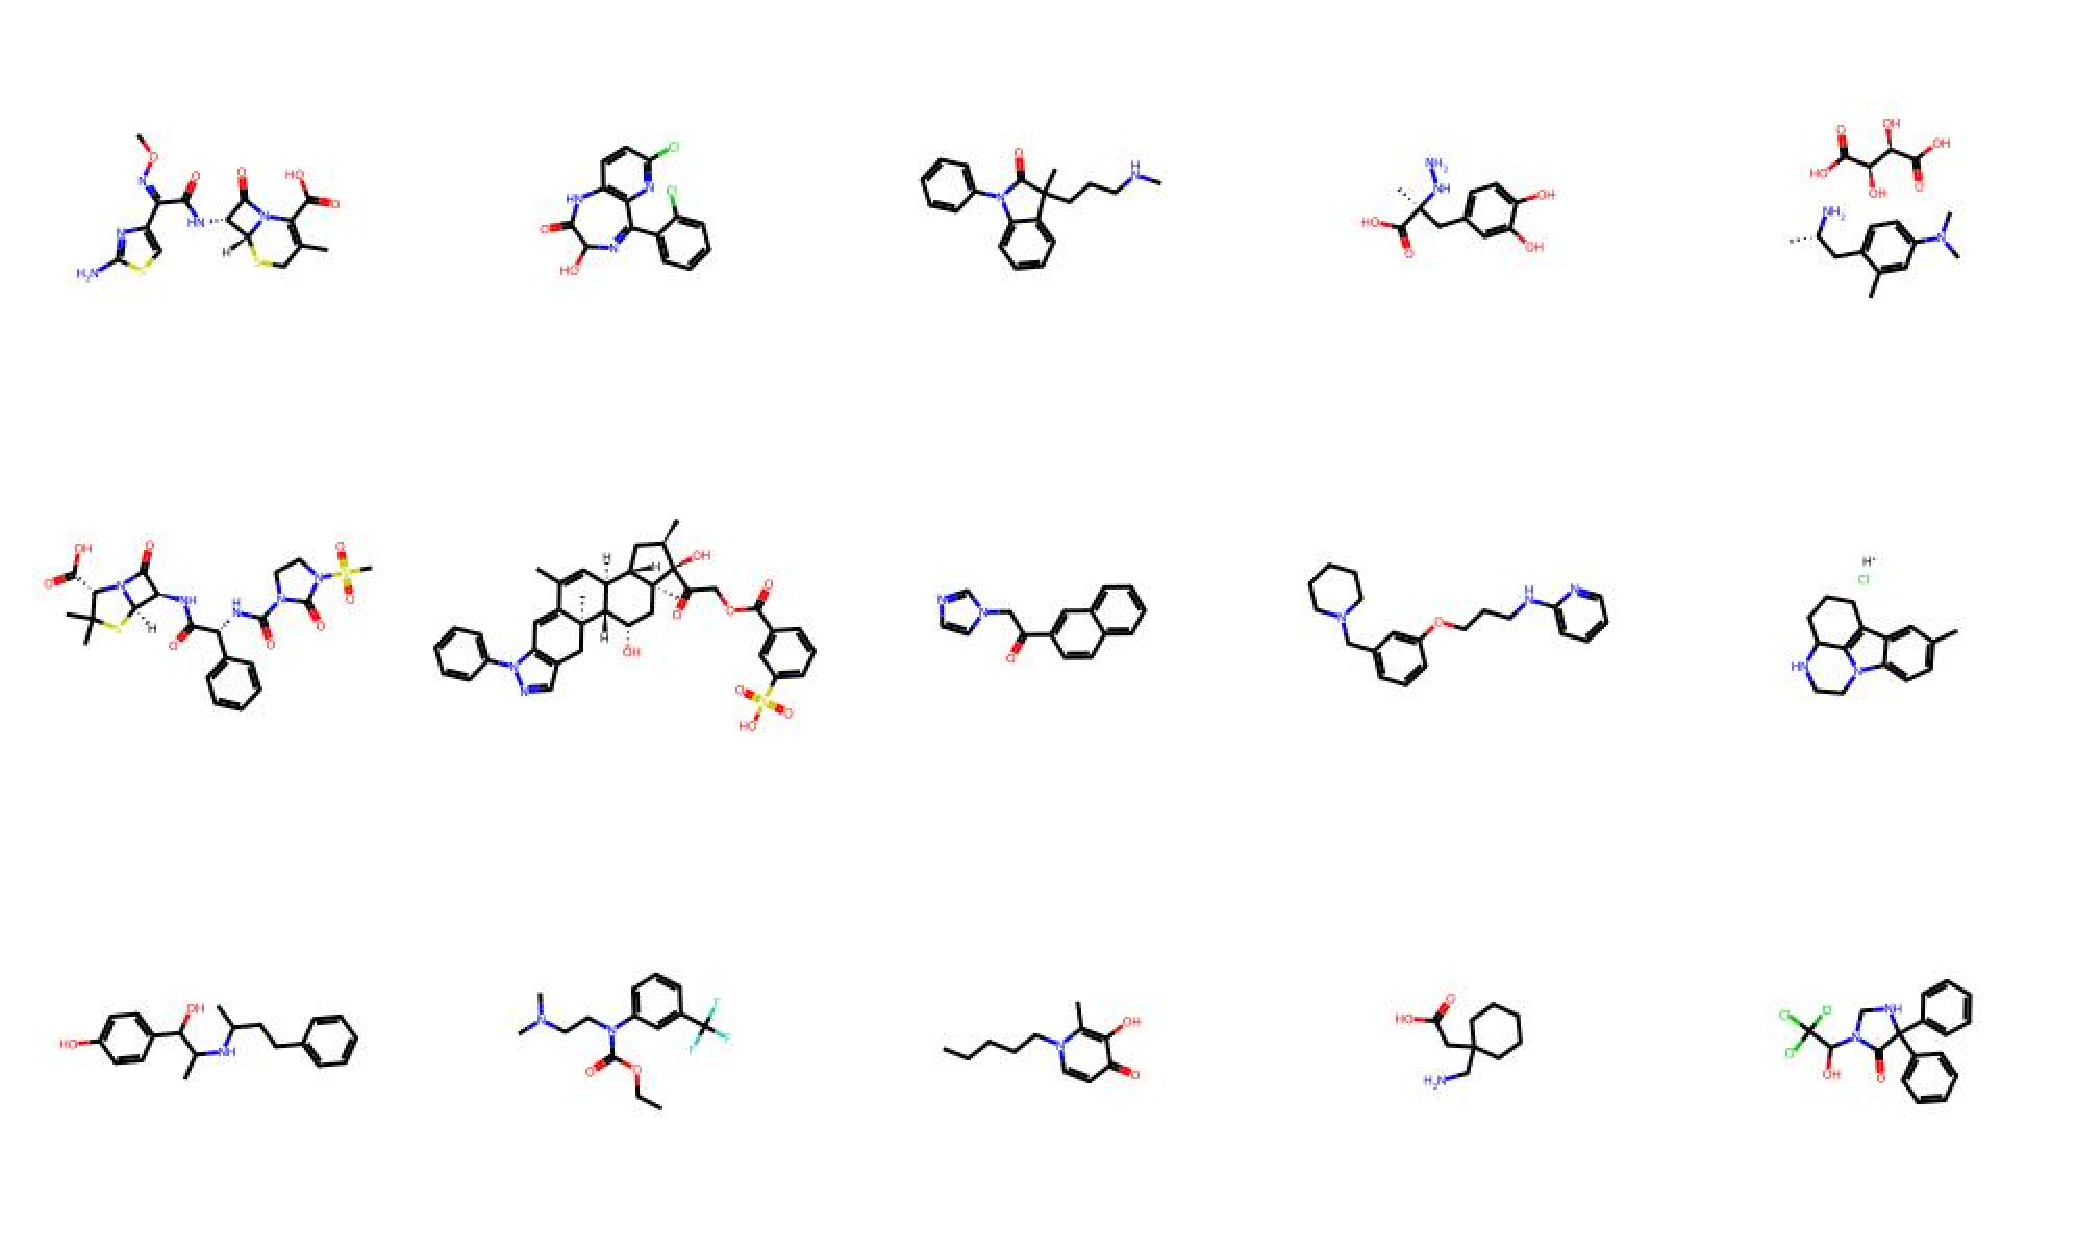
\includegraphics[width=\textwidth]{example_graphs.pdf}
    \caption{The graphs from the dataset in memory}
    \label{fig:examples}
\end{figure}

In terms of code files, our work on the data processing pipeline is summarized in Table \ref{tab:dataprocess}.

\begin{table}[ht]
\centering
\caption{Summary of our data processing pipeline and where they live in the codebase.}
\label{tab:dataprocess}
\begin{tabularx}{\textwidth}{ccX}
\toprule
\textbf{Directory in \texttt{model/}} & \textbf{Module} & \textbf{Description}\\
\midrule
\multirow{16}{*}{\textbf{utils/}} & \texttt{conversions} & \texttt{smile\_to\_graph} converts SMILE strings for a molecule into graphs. This is internally done with two helper functions to first convert a SMILE string to a molecule and then find out various properties of the molecule and then encodes them in a graph.\\
&\texttt{feature\_encoder}& \texttt{FeatureEncoder} is an abstract class that lays the structure for encoding molecular properties to graphs. \texttt{AtomFeatureEncoder} is a class inheriting from \texttt{FeatureEncoder} and encodes atom-level properties into the graph. \texttt{BondFeatureEncoder} is a class inheriting from \texttt{FeatureEncoder} and encodes bond-level properties into the graph.\\
&\texttt{apply\_feature\_encoder}& \texttt{atom\_feature\_encoder} creates an instance of the \texttt{AtomFeatureEncoder} class using the configuration. \texttt{bond\_feature\_encoder} creates an instance of the \texttt{BondFeatureEncoder} class using the configuration.\\
\midrule
\multirow{8}{*}{\textbf{dataset/}} & \texttt{download\_dataset} & Download the BBBP dataset and check if the dataset is corrupted.\\
&\texttt{download\_elements}& Download the Periodic table dataset and check if the data is corrupted.\\
&\texttt{loader}& \texttt{repeatx} is used to expand dimensions of a tensor. \texttt{merged\_batch} merges multiple data points to form a batch of data to be fed in. \texttt{loader} takes in multiple graphs and creates a TensorFlow Dataset from them. \texttt{split\_data} allows to easily split the dataset into a train, test, and validation set. \texttt{bbbp\_dataset} is a wrapper that splits the data.\\
\bottomrule
\end{tabularx}
\end{table}

\subsection*{Implementing a message-passing Neural Network}

Our project extensively makes use of the ideas Graph Neural Network \citep{4700287}. We think there is great potential for graph-based Machine Learning models as demonstrated by recent works like Message Passing Neural Networks \citep{gilmer2017neural}, Graph Convolutional Networks \citep{https://doi.org/10.48550/arxiv.1609.02907}, Graph Attention Networks \citep{https://doi.org/10.48550/arxiv.1710.10903} and GraphSAGE \citep{hamilton2017inductive}. Modeling chemical interactions with computational graphs and implementing machine-learning models, streamlines drug discovery tasks with in-silico simulations, greatly aiding research efforts in this area. In the past, there have been works exploiting this aspect of graph-based machine learning approaches like predicting protein interfaces by \cite{fout2017protein}.

On a high level, our message passing neural network model implementation can be reduced \citep{daglignns} to:
\begin{itemize}
    \item The node’s feature vectors are transformed using some sort of projection.
    \item They are aggregated by a permutation-invariant function.
    \item The feature vector of each node is updated based on its current values and the aggregated neighborhood representation.
\end{itemize}

We implement the neural message passing \citep{jorgensen2018neural, gilmer2017neural} in neural networks, specifically, we aim to closely mimic the ideas presented by \cite{jorgensen2018neural} in their work on predicting formation energy and other properties of molecules and materials. We will often use a force or convolution operator analog:
\begin{equation*}
    m\frac{\mathrm{d} \vec{v_i}}{\mathrm{d}t} = \sum_{j \in \textrm{ neighbours of } i } \vec{F}(\vec{r_i}, \vec{r_j}, e_{ij})
\end{equation*}
We utilize the notion of messages in GNNs. A message $m_{ij}$ can be sent across edges $i$ and $j$ and is parameterized using a message function $f_e$, which we implement as a neural network.
\begin{equation*}
    \vec{m_{ij}}=f_e(\vec{h_i}, \vec{h_j}, \vec{e_{ij}})
\end{equation*}
where $\vec{h_i}$ represents the node properties of node $i$ and $e_{ij}$ represents the edge properties of edge $ij$. We divert the reader to mainly see what comprises a single message which is analogous to filters in standard neural networks.

All messages arriving at each node are then aggregated using a permutation-invariant function, such as summation. The aggregated representation is then combined with the existing node features using a simple reparameterization trick as a neural network:
\begin{equation*}
    \vec{h_i^{\prime}} = f_v(h_i, \sum_{j \in N_i} \vec{m_{ij}})
\end{equation*}

Now to update the edge properties we use another neural network, $U_{edge}$:
\begin{equation*}
    e_{ij}^{\prime} = U_{edge}(e_{ij}, x_i, x_j)
\end{equation*}

In code, we implement this following the framework listed in Table \ref{tab:model}. Our model computation is visually summarized in Figure \ref{fig:computation}.

\begin{table}[ht]
\centering
\caption{Summary of our model training code and where they live in the codebase.}
\label{tab:model}
\begin{tabularx}{\textwidth}{ccX}
\toprule
\textbf{Directory in \texttt{model/}} & \textbf{Module} & \textbf{Description}\\
\midrule
\multirow{10}{*}{\textbf{train\_model/}} & \texttt{build\_model} &\texttt{EdgeNetwork} class is a TensorFlow layer that implements the edge update network earlier represented as $ \vec{h_i^{\prime}} = f_v(h_i, \sum_{j \in N_i} \vec{m_{ij}})$. \texttt{MessagePassing} class is a TensorFlow layer that implements Message passing throughout the network using the edge update layer defined. \texttt{TransformerEncoderReadout} class implements a standard Attention layer as shown in \cite{vaswani2017attention} to get the final brain membrane permeability from the graph. \texttt{PartitionPadding} class implements adding padding to molecules to compensate for varying numbers of atoms in a molecule. \texttt{create\_model} function brings this together building a TensorFlow model using the Functional API.\\
\bottomrule
\end{tabularx}
\end{table}

\begin{figure}[htbp]
    \centering
    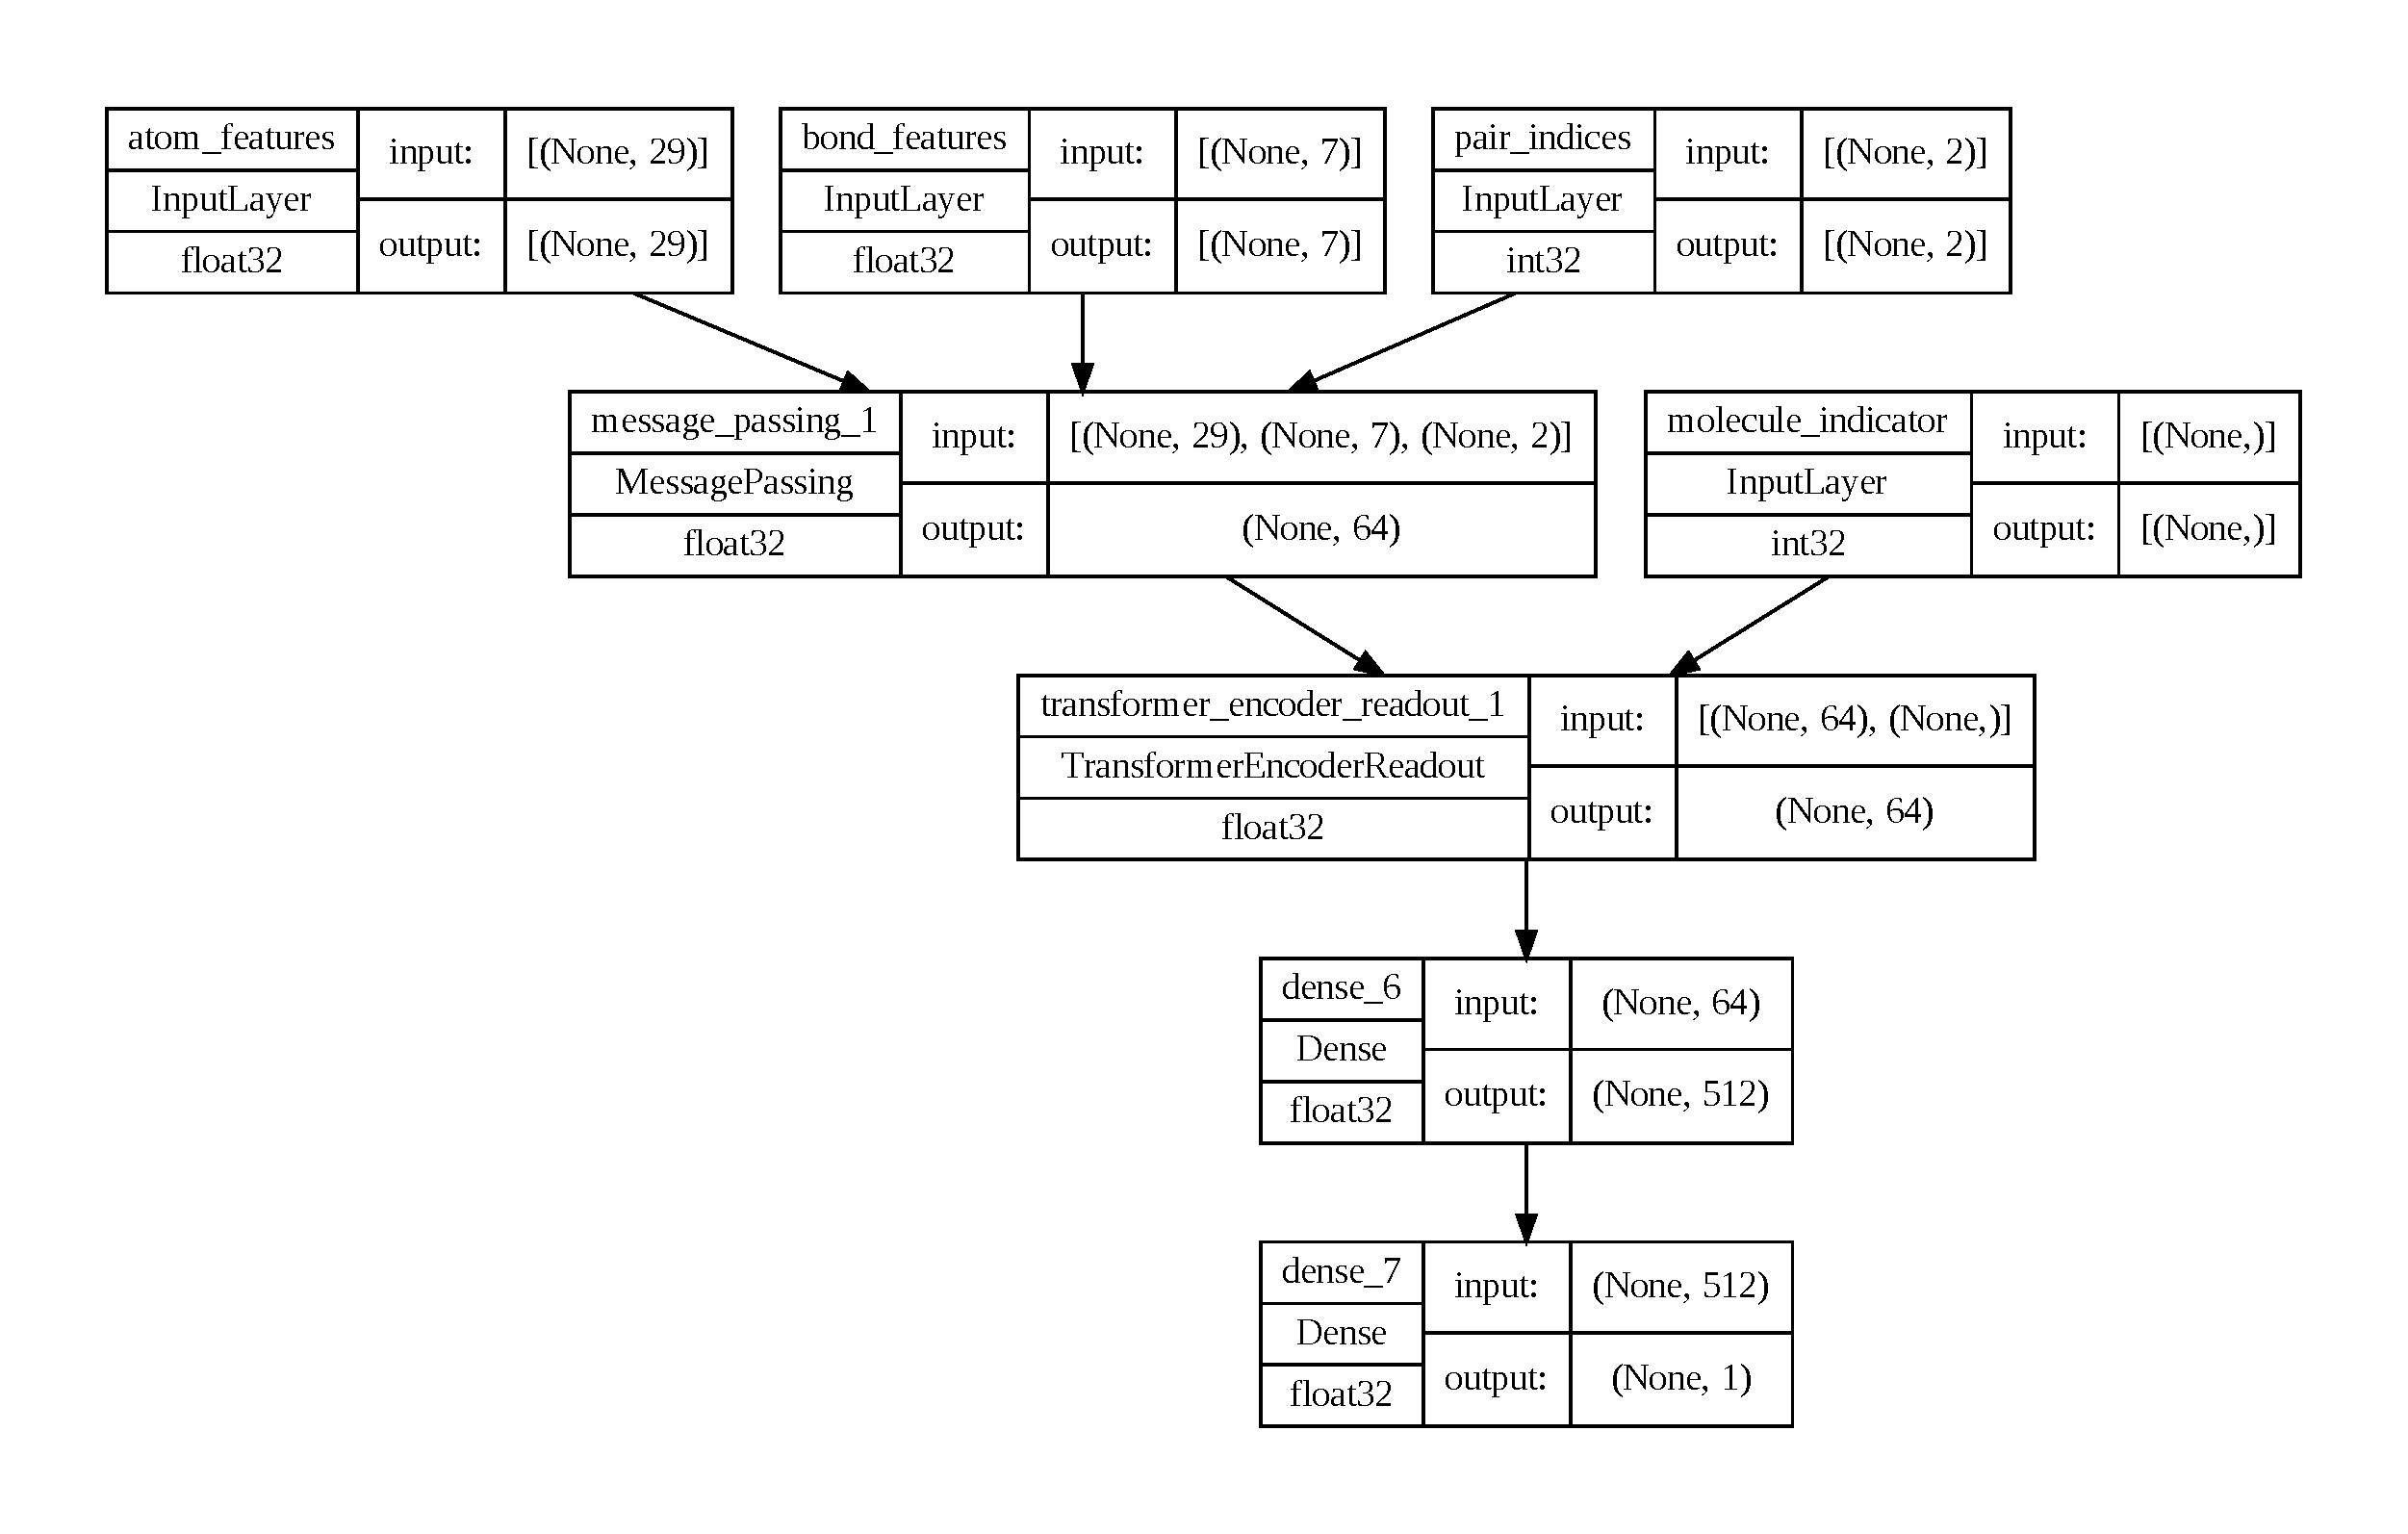
\includegraphics[width=\textwidth]{computation.pdf}
    \caption{Our Model computation summarized on a high-level.}
    \label{fig:computation}
\end{figure}

\subsection*{Training the Model}

Training the model after implementing message passing neural network is now rather straightforward and is summarized in table \ref{tab:train}.

\begin{table}[ht]
\centering
\caption{Summary of our model training code and where they live in the codebase.}
\label{tab:train}
\begin{tabularx}{\textwidth}{ccX}
\toprule
\textbf{Directory in \texttt{model/}} & \textbf{Module} & \textbf{Description}\\
\midrule
\multirow{3}{*}{\textbf{training/}} & \texttt{train} &\texttt{create\_and\_train}function brings the model created earlier to train it with the configuration specified in \texttt{model/configuration/training.py} and implements logging and hardware accelerator specific code for the model training as well.\\
\bottomrule
\end{tabularx}
\end{table}

\subsection*{Training Results}

Since most of our projects involved training a model, we include our model training results, to foster easy reproducibility of these models, not just the model weights and training code being released but also include the training logs and the exact configurations used to reproduce these results.

We spent quite some time searching for the best hyperparameters to train the model, all the training logs and accompanying search results can be found at 
 this TensorBoard URL \footnote{\url{https://tensorboard.dev/experiment/MUl2ENlaS2mMjxzSw1nG5g/}}. The training logs for the final deployable model can be found at this tensorBoard URL\footnote{\url{https://tensorboard.dev/experiment/MUl2ENlaS2mMjxzSw1nG5g/}} with which we were able to get to $0.93$ AUC on the test-split.

In Figure \ref{fig:training_logs} we demonstrate the training progress of the model and through Figure \ref{fig:scaling_logs} we attempt to justify the need for the extensive hyperparameter tuning we perform.

\begin{figure}[htbp]
  \centering
  \begin{minipage}{0.45\textwidth}
    \centering
    \includesvg[width=\linewidth]{epoch_loss.svg}
    \subcaption{}
  \end{minipage}\hfill
  \begin{minipage}{0.45\textwidth}
    \centering
    \includesvg[width=\linewidth]{epoch_AUC.svg}
    \subcaption{}
  \end{minipage}
  \caption{The training curves for (a) cross-entropy loss, lower is better and (b) area under the curve, higher is better, with respect to the number of epochs.}
  \label{fig:training_logs}
\end{figure}

\begin{figure}[htbp]
  \centering
  \begin{minipage}{0.45\textwidth}
    \centering
    \includesvg[width=\linewidth]{scaling_loss.svg}
    \subcaption{}
  \end{minipage}\hfill
  \begin{minipage}{0.45\textwidth}
    \centering
    \includesvg[width=\linewidth]{scaling_AUC.svg}
    \subcaption{}
  \end{minipage}
  \caption{The scaling curves for (a) cross-entropy loss, lower is better and (b) area under the curve with respect, higher is better, to the number of epochs, the full legend for these scaling curves can be found on the project's TensorBoard page. This particularly shows tuning hyperparameters for this problem was immensely helpful.}
  \label{fig:scaling_logs}
\end{figure}

We could most certainly have built a better-performing model by building a model using some modern deep learning techniques but considering the time and the scope of this project and the performance we were able to get from a small model we think this model makes for a good one for this project.

\subsection*{Inference}

The web application only uses the trained model from the earlier steps to infer from it. Having ended up with quite a large model, which we spent time training on and understanding the quirks for, optimizing this model was of the essence and we were also able to introduce optimizations to it using multiple optimizations from Grappler \citep{48051}. The way this is implemented in code is summarized in Table \ref{tab:infer}.

\begin{table}[ht]
\centering
\caption{Summary of our model inference code and where they live in the codebase.}
\label{tab:infer}
\begin{tabularx}{\textwidth}{ccX}
\toprule
\textbf{Directory in \texttt{model/}} & \textbf{Module} & \textbf{Description}\\
\midrule
\multirow{2}{*}{\textbf{inference/}} & \texttt{load\_model} &\texttt{download\_model} downloads the models and checks if the model is corrupted. \texttt{load\_model} function loads the downloaded TensorFlow model.\\
\midrule
\multirow{2}{*}{\textbf{inference/}} & \texttt{infer} &\texttt{predict} function converts entered SMILE string to a graph and passes it through the model to get a prediction.\\
\bottomrule
\end{tabularx}
\end{table}

\subsection*{Packages Used}

We use the following packages apart from the ones taught in the course:
\begin{itemize}
    \item TensorFlow \citep{abadi2016tensorflow} for making it a bit easier to implement the machine learning models and training processes without having to worry about fundamental tensor handling and autodiff
    \item TensorFlow-GNN \citep{ferludin2022tf} for implementing machine learning in the graph-based setting
    \item RDKit \footnote{\url{https://www.rdkit.org/}} for cheminformatics and handling SMILES strings
    \item einops \citep{rogozhnikov2022einops} for implementing multiple operations using Einstein notations
    \item Numpy \footnote{\url{https://numpy.org/}} for working with scientific computations
    \item Streamlit \footnote{\url{https://streamlit.io}} for creating the web app and integrating HTML, and CSS within Python
\end{itemize}

\section*{Instructions for Obtaining Datasets and Running the Project}

The requirements.txt file mentions all the python libraries that will be required to run this project. We have mentioned all the libraries that have been used to train and test the model, and also all the libraries required to load the model as part of running our project. Furthermore, our program will also require you to install streamlit version 1.20.0 to create and run the web app. Lastly, we have also used python-ta for testing and checking the correctness of our code. Alternatively, you can run the following command in the terminal to install all dependencies for this project:

\begin{verbatim}
    pip install requirements.txt
\end{verbatim}

There are 2 ways to run our project, one where you can train the model yourself and the other where you can run the model that we have pre-trained and run the project with it.

\subsection*{Running the App}
Our submission for the final project includes a zip folder containing all the files that are required for running our project. This folder contains the \texttt{requirements.txt}, \texttt{main.py}, other files created for running the project, and all the files of the machine learning model as well. Once you extract all the files from the zipped folder, you need to open the project on PyCharm and run the \texttt{main.py} file with the following \texttt{streamlit run} command:

\begin{verbatim}
    streamlit run main.py
\end{verbatim}

This should open the streamlit web app in your browser which should look like the figure given below. This is the homepage of our web app that contains the basic information about our project and the instructions to us the web app.

\begin{figure}[ht]
    \centering
    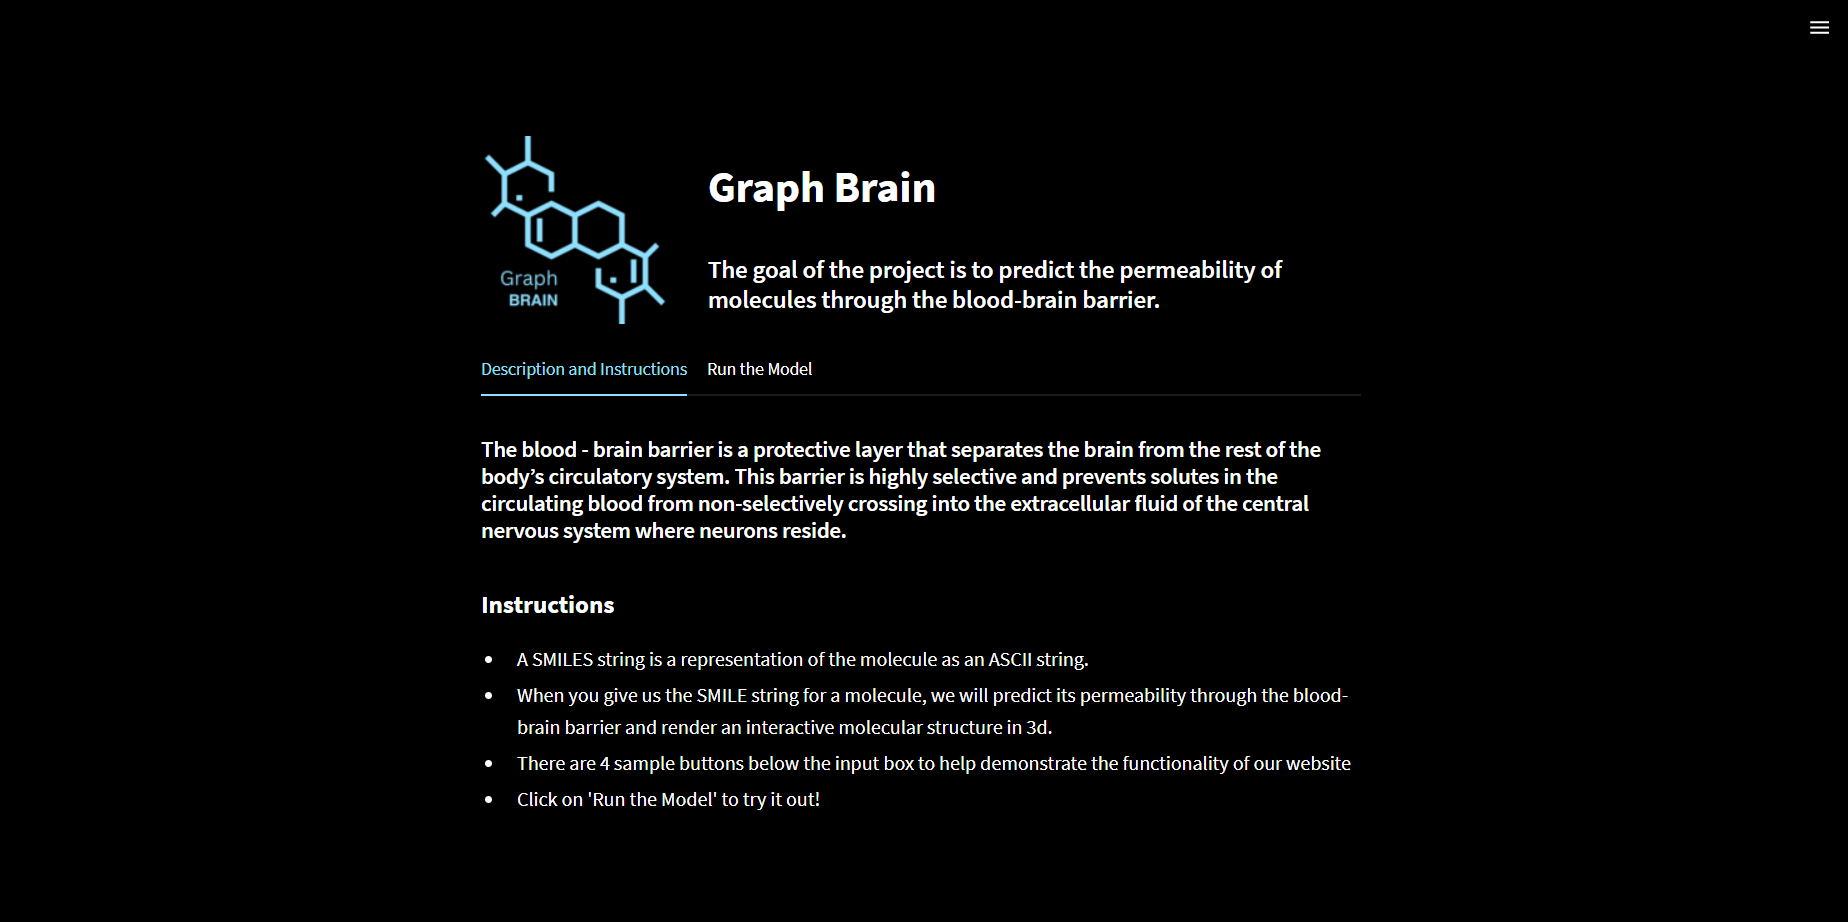
\includegraphics[width=0.8\textwidth]{webapp1.png}
    \caption{Home Page of the website}
    \label{fig:homepage}
\end{figure}

There is a separate page for running the model which should look like Figure 2

\begin{figure}[ht]
    \centering
    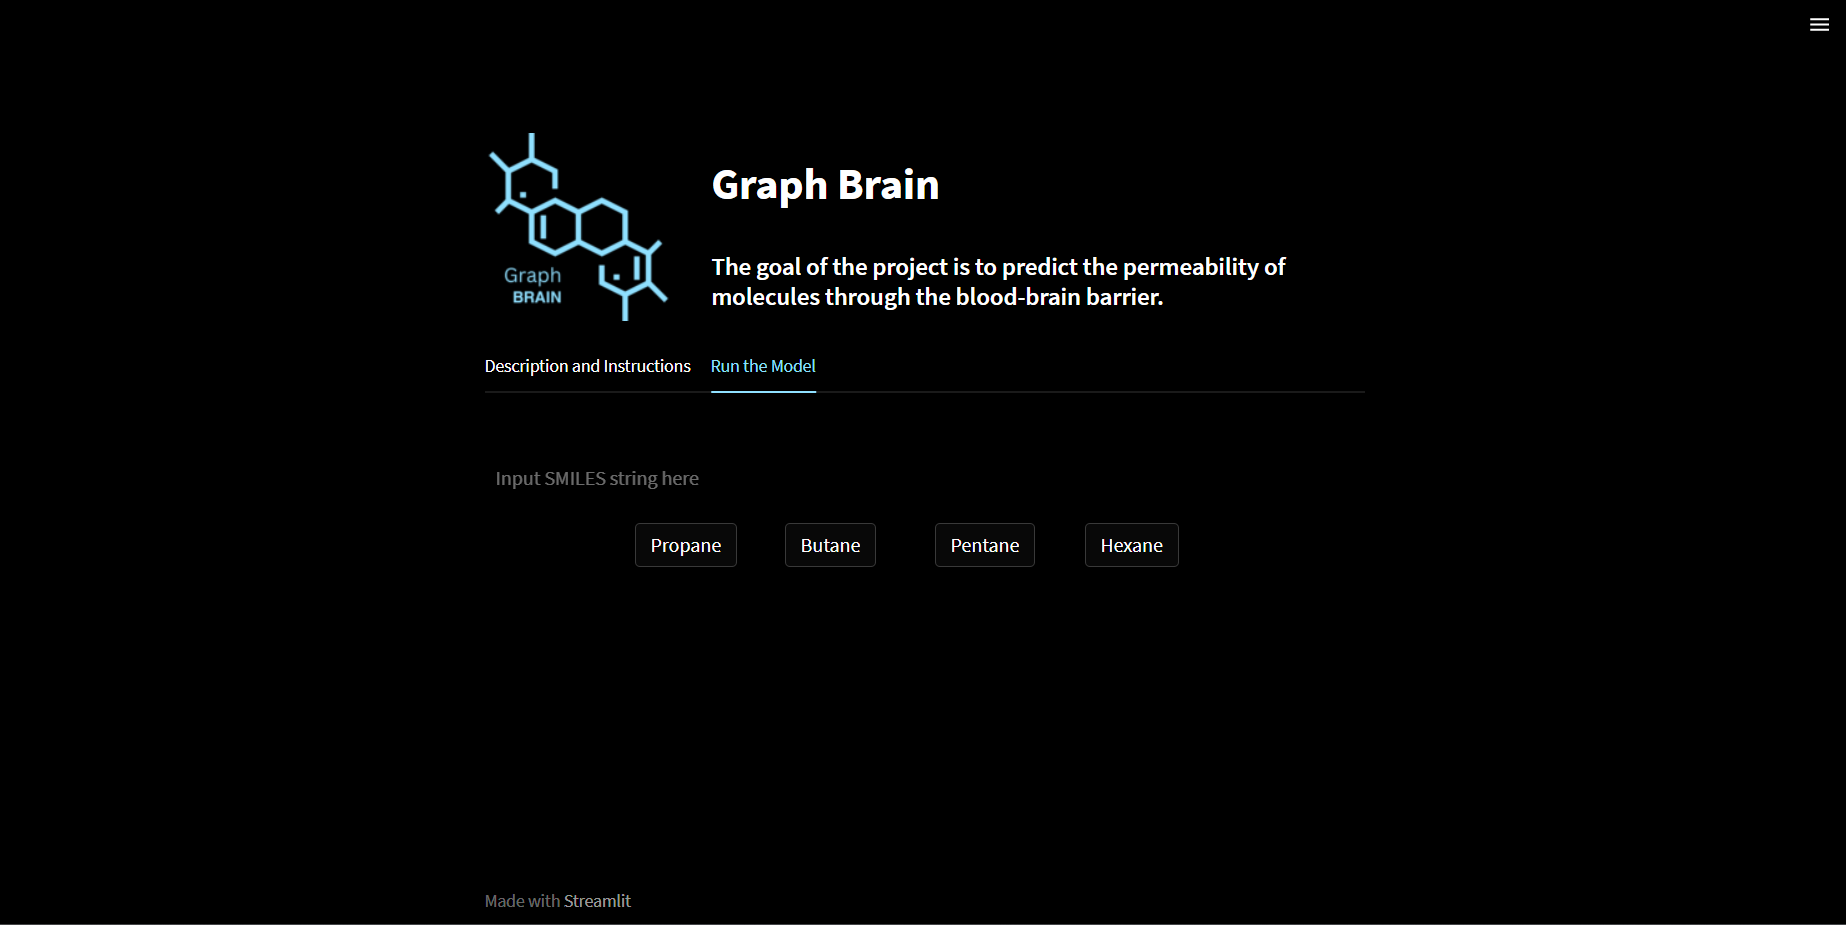
\includegraphics[width=0.8\textwidth]{webapp2.png}
    \caption{Model Page}
    \label{fig:modelpage}
\end{figure}

In order to run the model you need a SMILES string of the molecule whose permeability is to be predicted. A SMILES string is a representation of the molecule as an ASCII string. Once you input the SMILES string and press enter, we will predict its permeability through the blood-brain barrier and render an interactive molecular structure in 3d. There are 4 sample buttons below the input box to help demonstrate the functionality of our website.

Now, let's say you want to know the blood-brain barrier permeability of alcohol. You can enter the SMILES string \textbf{CCO} in the input box and our model will generate a 3d rendering of the molecule of alcohol and display its permeability value. This is what the webapp should look like:

\begin{figure}[ht]
    \centering
    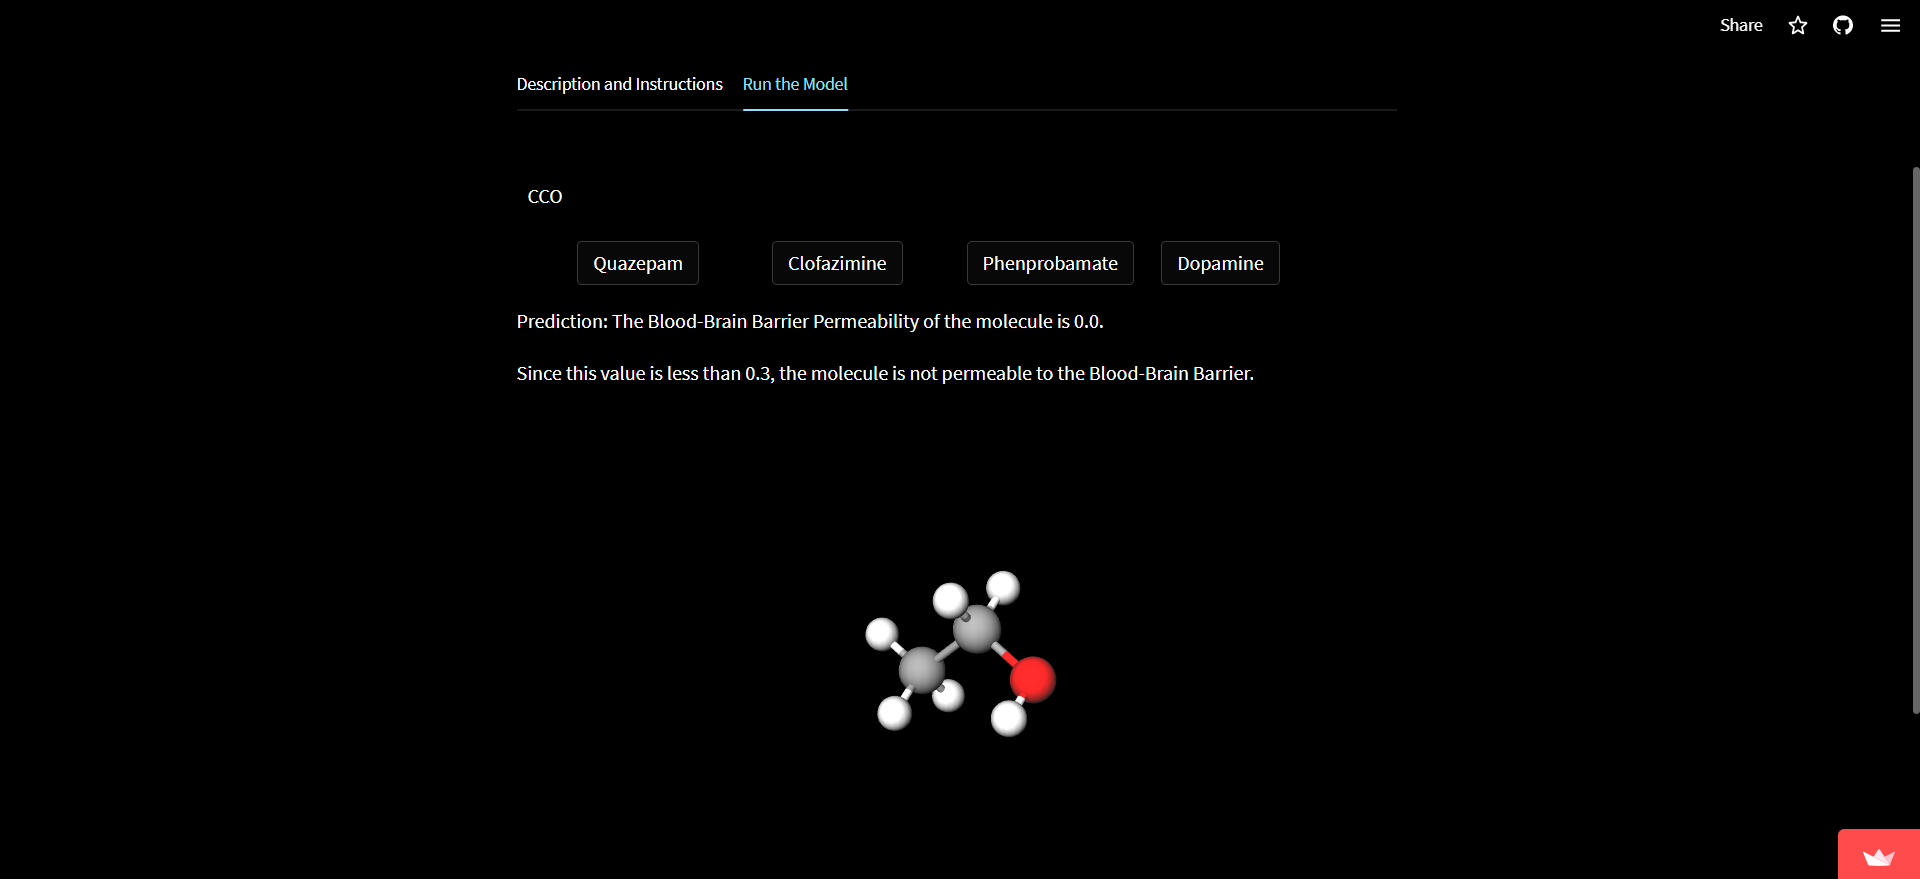
\includegraphics[width=0.8\textwidth]{webapp3.png}
    \caption{Expected Result}
    \label{fig:visualizeaugmentations}
\end{figure}

\subsection*{Training the model}

This step is not required to run the application, running the application just takes artifacts from the training step and uses those. This section describes how one would train the model from scratch.

\paragraph{Modifying the configuration:} The first step in training any model is modifying the configuration for the training. The configuration file is present at \texttt{model/configuration/training.py}. This file dictates how the training takes place and any options. We provide a sample configuration to add the graders in quickly running a single training epoch on a CPU. However, one could easily make changes to this file to do the full training (as described later this last for $300$ epochs), if the grader plans to do the full training, we suggest using at least 4 GPUs or a TPU pod.

\paragraph{Training the Model:} Once any changes to the configuration (if required) are made we would need to install a library to create model plots (this installation is only required if \texttt{"plot\_model": True,} is present in the configuration):

\begin{verbatim}
    sudo apt-get update
    sudo apt install graphviz
\end{verbatim}

Once we do this we are ready to train the model by running:

\begin{verbatim}
    python model/training/train.py
\end{verbatim}

Based on the configuration and the hardware this step could take quite some while however a single epoch on a CPU (default configuration) would not take more than 10 minutes to run.

\paragraph{Artifacts:} Once this is run, it saves the training logs in a newly created directory \texttt{logs/fit/unique\_identifier} and saves the trained model at \texttt{logs/fit/unique\_identifier/model}. All the results and computations shown in the Computational Overview section are reproducible using the aforementioned instructions.

\subsection*{Obtain the Datasets}

As we mentioned above, the data we used for this project is readily available as a part of MoleculeNet \citep{wu2018moleculenet} which contains 2,050 molecules and each molecule comes with a name, label, and SMILES string. We also use the Periodic Table dataset introduced by \cite{periodicdataset} which contains a mapping from the element names to their symbols. We have provided both the datasets we are using as \texttt{.csv} files in the zip folder submitted on MarkUs. These datasets were used for training the model we've used as part of our project and therefore have no direct functionality in running the application. However, these can be used to train our model and have a better idea of how our project works.

\section*{Changes from Original Plan}

While the overall structure and implementation of our project is very similar to the original proposed plan, one of the changes to our plan is the modification of our goal statement. We had proposed that we would be predicting the permeability value of a given molecule, now we are specifying both the permeability value of the molecule as well as whether the molecule is permeable or not based on the value predicted by our model. Our model predicts a real number value between 0 and 1, a molecule is said to be permeable if the value is $\geq$ 0.3. Thus, we will output both the predicted permeability value and whether the molecule is permeable or not. The datasets we have used are same as mentioned in the proposal and are also mentioned in the report. Lastly, while most of our computational plan is the same as we proposed, we had received a feedback to not use WASM, we decided not to use WASM. Other than that, all the other aspects of our computational plan is the same. Finally, we also decided to name our project \textbf{GraphBRAIN}.

\section*{Discussion}

Our project aimed to develop a machine learning model to predict the blood-brain barrier permeability of a given molecule using the BBBP dataset by MoleculeNet. Our results demonstrate that we have been successful in achieving this.

We found that a range of factors, such as molecular weight, number of rotatable bonds, number of hydrogen bond donors, ionizability, electronegativity, molecular size, play a role in blood-brain barrier permeation. We took into account all these factors by drawing out diagrams of the molecular structures. Keeping in mind their stereochemistry and using machine learning algorithms, we were able to develop a model which accomplishes the task with high accuracy and precision.

Our results provide important insights into the complex mechanisms underlying blood-brain barrier permeability and demonstrate the potential of machine learning in drug research and development. By using our model, researchers can rapidly screen large numbers of potential drug candidates and focus their efforts on those with the greater affinity to cross the blood-brain barrier.

The ability to predict blood-brain barrier permeability has significant implications for drug development. Particularly for the treatment of brain disorders such as Alzheimer's disease and Parkinson's disease. Identifying compounds that can effectively cross the blood-brain barrier and target the central nervous system is crucial for developing new and more effective treatments for these and other neurological disorders. It will also help prevent use of chemicals which might cross the blood-brain barrier unwantingly.

Traditional methods for determining blood-brain barrier permeability are time-consuming, expensive, and often require specialized expertise. By contrast, our machine learning approach can rapidly analyze large amounts of data accurately. Thus we feel our project has been successful in achieving its goal.

Talking about limitations and obstacles, one of the major limitations we faced in training our model was the limited quantity of datasets we had at our disposal. While the quality of the datasets we used was very good, it was the quantity that limited us in training our model. The dataset we used had only data of about 2050 molecules in total. Training our model on limited data meant it would not be perfect and accurate a hundred percent of the times, and we have found this to be the case for some complex unpredictable molecules. There might be some exceptional cases where the molecule is expected to be non-permeable through the blood-brain barrier, but the model might predict it as being permeable. 

Another problem we faced while implementing the UI od the website was figuring out how we could embed a 3D view of the molecule on the website. We wanted to include an interactive part to the website by integrating a 3D view of the molecule given by the user, but we faced a lot of difficulties while trying to implement this. We tried multiple software like rdkit and Indigo, but all of these implementations failed. Finally, we used MolView to implement this feature and were able to figure out how to correctly embed it in our website.

Also, while writing the code, we had written most of our code on a MacOS device thus the file paths and directories we used were relative to MacOS. Later, when we tried running the project on a Windows device, we realized that it was causing the website to fail because the file paths couldn’t be recognized. Thus, we had to go back and make the appropriate changes in our code so that it would be compatible with any operating system.

While there were a few more minor obstacles we encountered while working on this project, we were able to deal with them and implement our website successfully. 

In this project, we have successfully developed a machine learning model to predict the blood-brain barrier permeability of small molecules. However, there are still some areas that can be further explored to improve the model's accuracy and generalizability.

Firstly, although the current model achieved a relatively high accuracy on the test set, there is still room for improvement. One possible approach is to incorporate more diverse chemical descriptors, such as topological indices, pharmacophore features, and quantum chemical properties, into the feature set to capture a wider range of chemical properties that contribute to BBB permeability.

Additionally, the current study only used a single dataset for model training and evaluation. It would be valuable to test the model's performance on other independent datasets with different molecular structures and properties, to evaluate the generalizability of the model.

Lastly, the model must go through several rounds of testing before being used for research. Improving on exceptional and edge cases will prove very useful to our model.

In conclusion, the development of a machine learning model for predicting blood-brain barrier permeability has significant implications for drug discovery and development. Further exploration and refinement of the model can improve its accuracy, generalizability, and practical utility, and facilitate the discovery of novel central nervous system drugs with high efficiency.

\section*{Our Experience in The Area}

We were advised by Professor Mario Badr that we should add the previous experience we have with working on these kinds of projects and with the libraries since it might come off as a larger project.

\paragraph{Rishit Dagli} is currently researching machine learning and computer vision at the DGP Lab. In the past, he has been the primary author of multiple machine learning research works published/ accepted at Nature, ICLR 2023, and ACM SIGGRAPH among others. He has also served as a reviewer/program committee at top conferences like CVPR and ICLR. Earlier he also worked as an AI researcher at Google AI and at NASA JWST. He is also a maintainer of TensorFlow and has been a very active contributor to WebAssembly.

\paragraph{Shivesh Prakash} is a member of Professors David Lindell and Kyros Kutulakos' Toronto Computational Imaging Group at the DGP Lab. He is also working on University of Toronto Aerospace Team's FINCH satellite mission, focused in resolving smile and keystone distortion using machine learning techniques and algorithms.

\paragraph{Tanmay Shinde} has some experience working with graph infrastructures in the past. Previously, he has completed online machine learning and AI courses and is equipped with the basics of neural networks, churn modeling, and reinforcement learning with pandas, TensorFlow, cv2, and other python libraries. 

\paragraph{Pranjal Agrawal} has completed online machine learning courses.

\section*{Supplementary Figures}

Here we have compiled a few images of how the project works in certain cases, such as giving it a simple molecule, a complex molecule, and an invalid SMILES string.
\begin{figure}[h!]
    \centering
    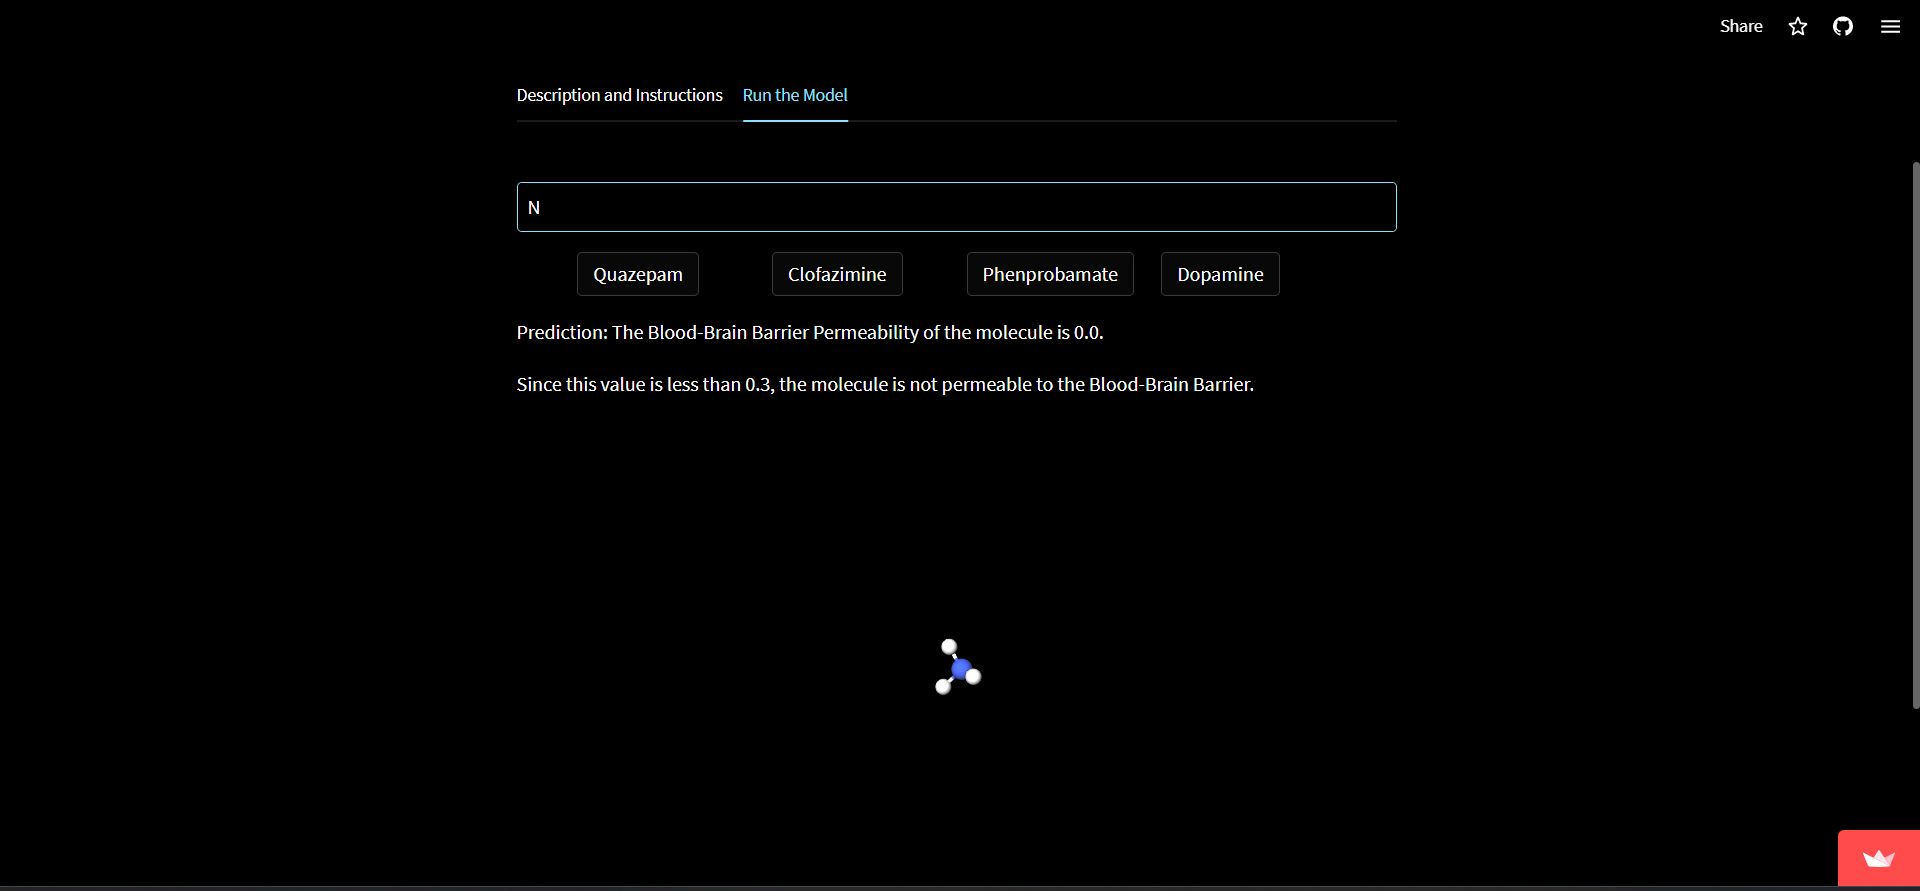
\includegraphics[width=0.8\textwidth]{ammonia_simple.png}
    \caption{Ammonia, a non-permeable molecule}
    \label{fig:ammonia}
\end{figure}

\begin{figure}[h!]
    \centering
    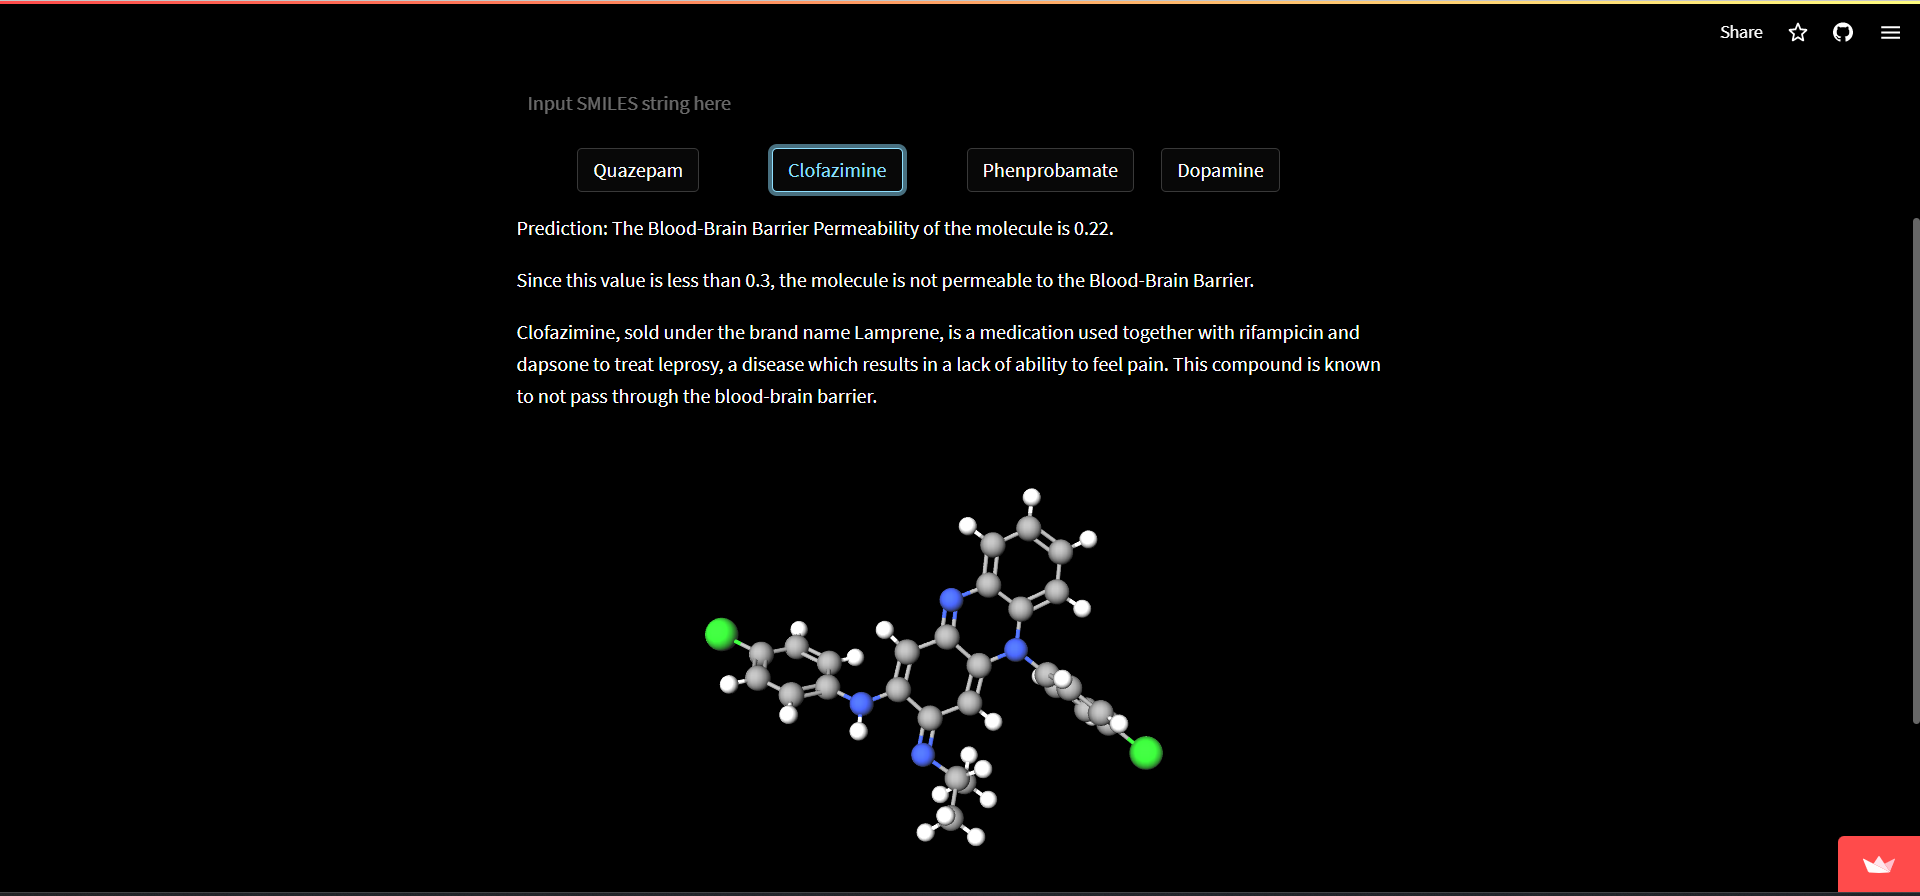
\includegraphics[width=0.8\textwidth]{example_clofazimine.png}
    \caption{Clofazimine, a non-permeable molecule, example button}
    \label{fig:clofazimine}
\end{figure}

\begin{figure}[h!]
    \centering
    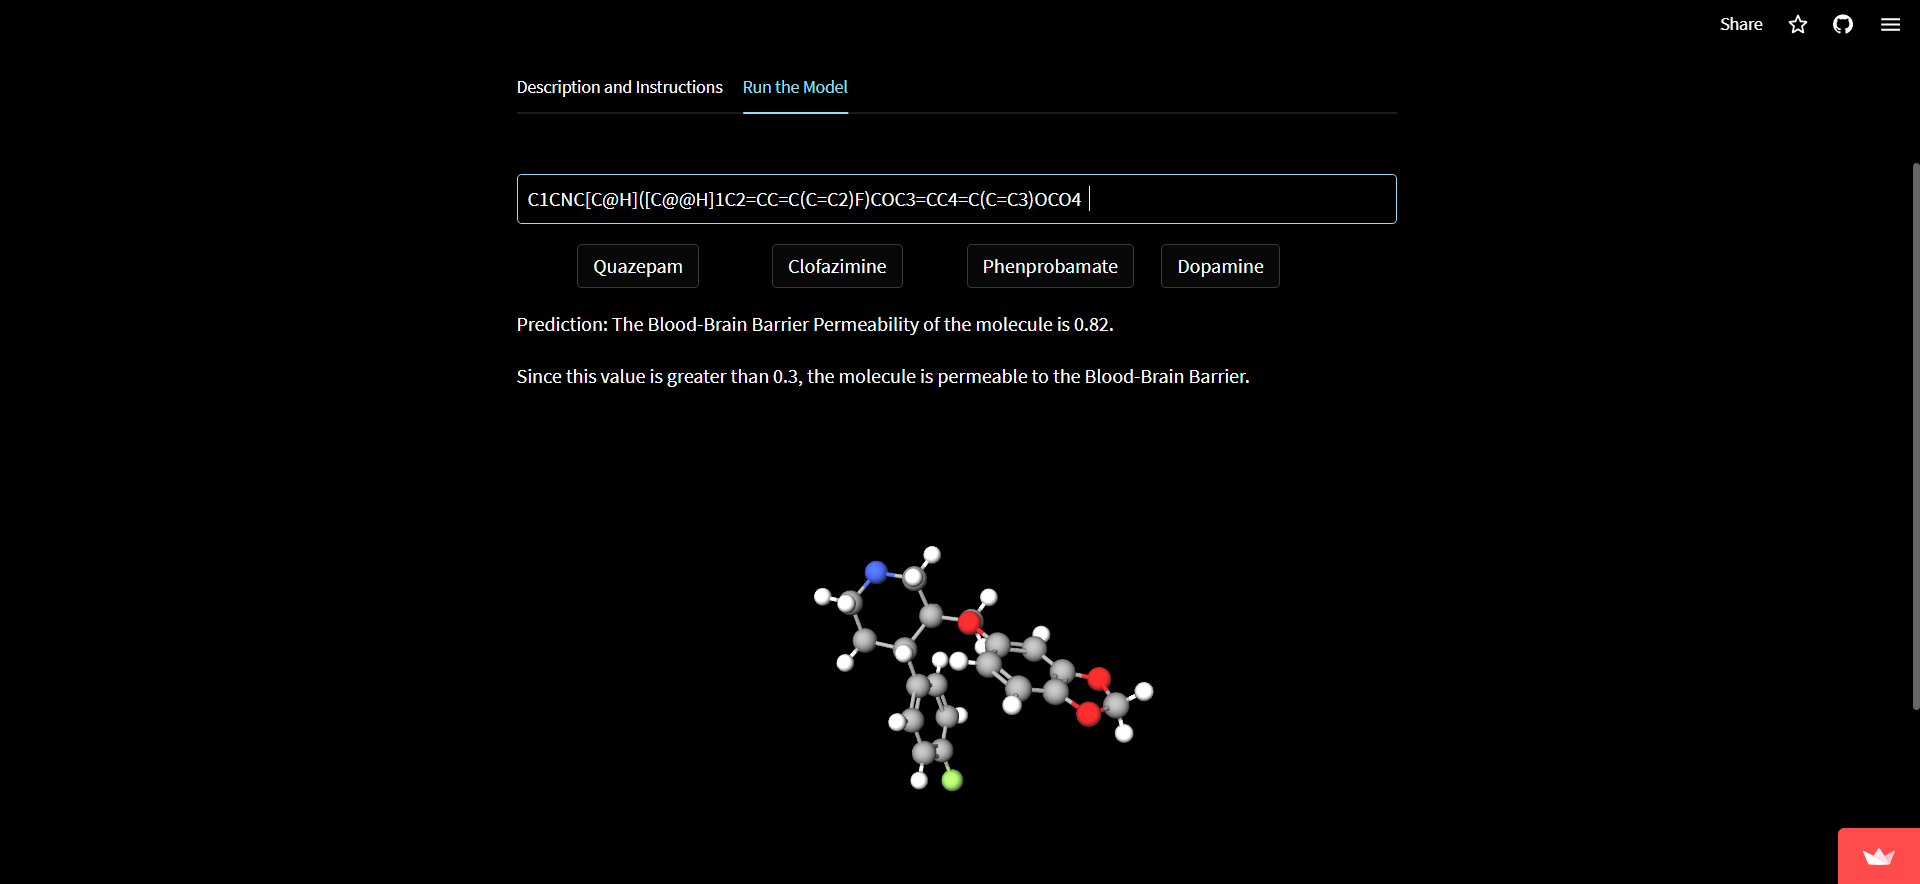
\includegraphics[width=0.8\textwidth]{complex_p_paroxetine.png}
    \caption{Paroxetine, a complex permeable molecule}
    \label{fig:paroxetine}
\end{figure}

\begin{figure}[h!]
    \centering
    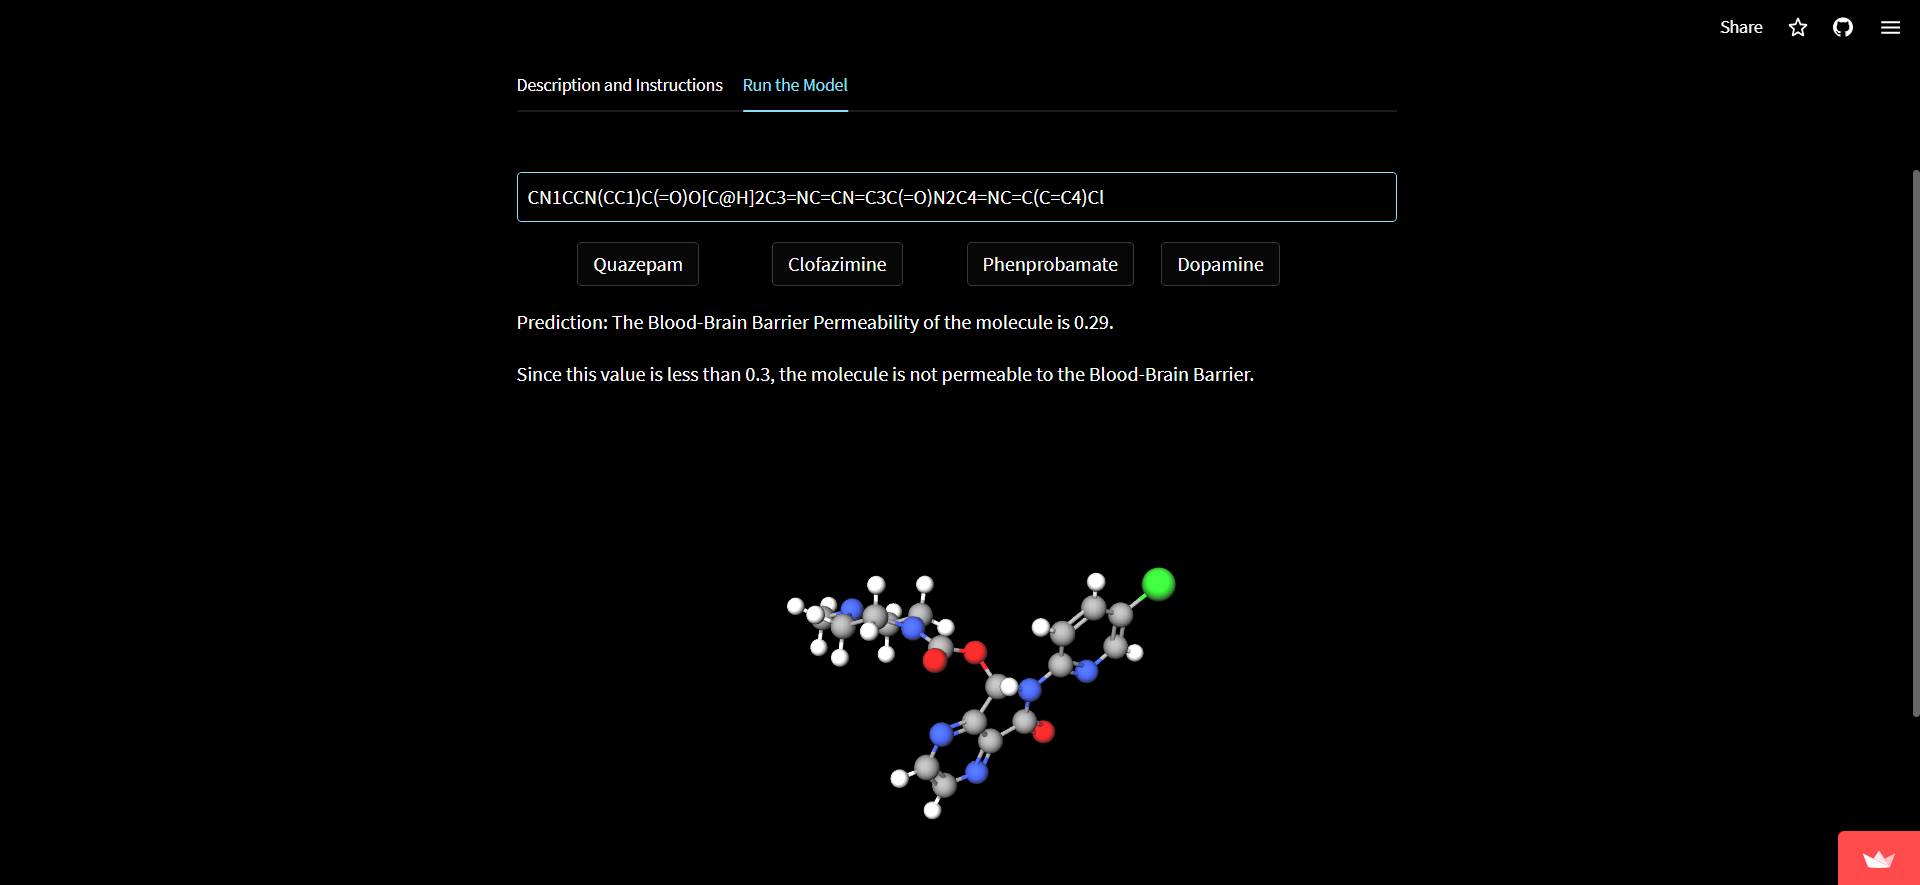
\includegraphics[width=0.8\textwidth]{complex_np_eszopiclone.png}
    \caption{Eszopiclone, a complex non-permeable molecule}
    \label{fig:eszopiclone}
\end{figure}

\begin{figure}[h!]
    \centering
    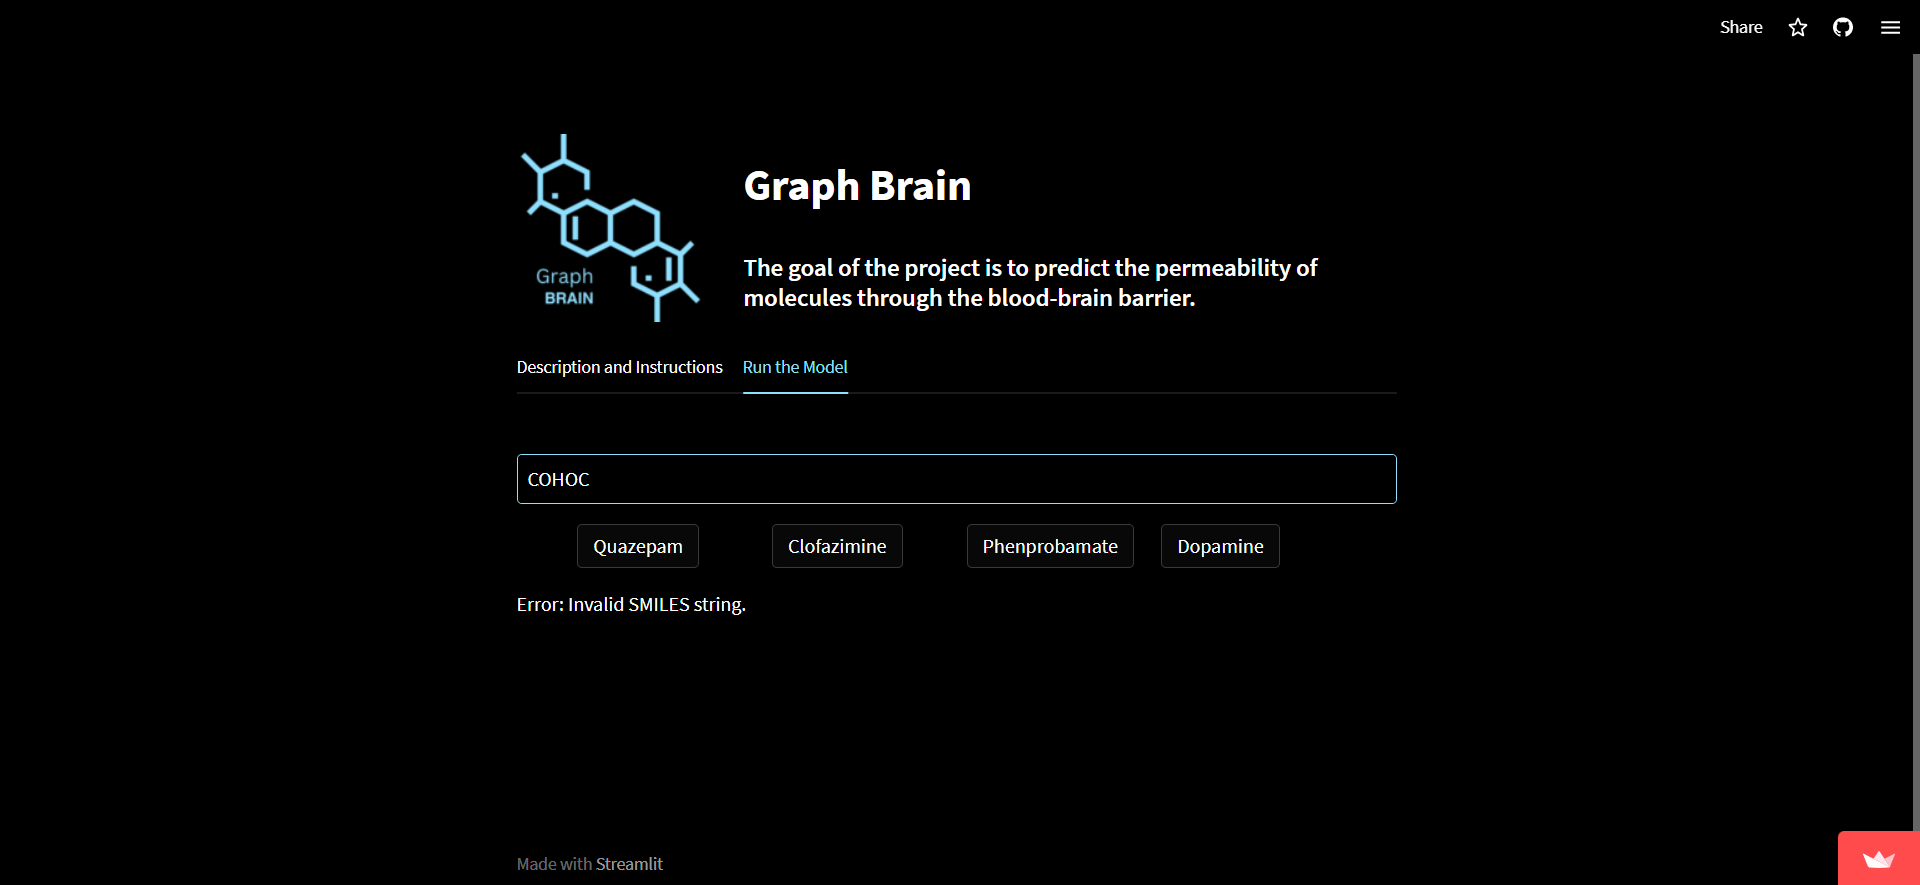
\includegraphics[width=0.8\textwidth]{invalid.png}
    \caption{Invalid SMILES string}
    \label{fig:invalid}
\end{figure}
\newpage
\bibliography{references}

\end{document}